\section{Filter}
Die Filter-Charakteristik kann mithilfe der Übertragungsfunktion $H(s)$ beschrieben werden. Die DC-Verstärkung kann bei $H(0) = \text{DC}$ erhausgelesen werden. 

Die \textbf{Kreisgüte} $Q$, mit Verstärkung $A_0$ und Kreisfrequenz $\omega_0$. Die entsprechenden Werte können durch \textbf{Koeff.vergleich} berechnet werden. Allgemeine Form für 2. Ordnung:
\[
H(s) = \frac{\omega_0^2 \cdot A_0}{s^2 + \frac{\omega_0}{Q}s + \omega_0^2} = \frac{A_0}{\frac{1}{\omega_0^2}s^2 + \frac{1}{Q\cdot \omega_0}s + 1}
\]

Passive Bauelemente können Güten maximal bis $0.5$ erreichen. Filter höherer Güte benötigen entweder Spulen oder Verstärker. \textbf{Hinweis:} Übertragungsfunktionen können schnell mit Knotenpotential-Methode gefunden werden.

\subsection{Bode}
Siehe Kapitel \ref{approx_bode}

\subsection{Hochpass}
\begin{minipage}{0.20\textwidth}
	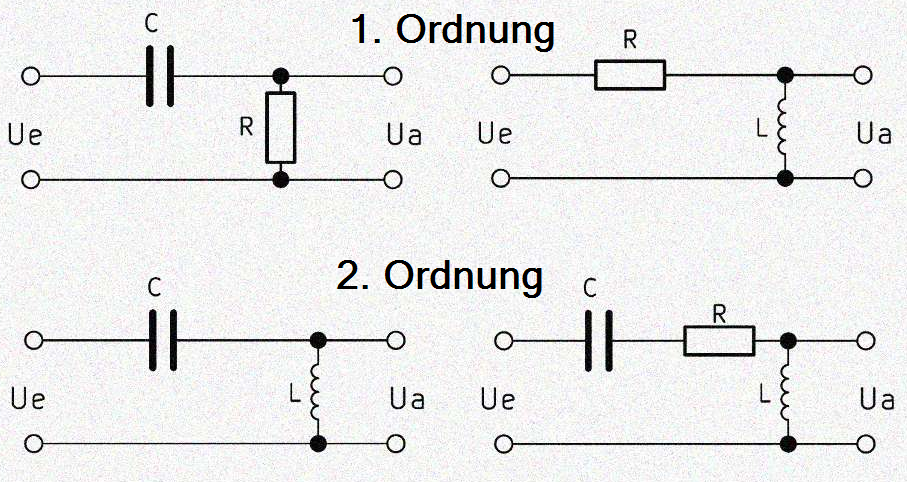
\includegraphics[angle=90,origin=c,width=0.8\linewidth,keepaspectratio=true]{./Images/filter_hochpass}
\end{minipage}%%% to prevent a space
\begin{minipage}{0.30\textwidth}
	Hochpass-Filter lässt hohe Freuenzen durch und filtert tiefe raus. Die allgemeine UTF für 1. Ordnung mit CR Komponenten:
	\[
	\frac{RCs}{\underbrace{RC}_{\tau}s + 1}
	\]
	Der Bode $3dB$ Knick (Real- und Imaginärteil gleich gross, entspricht Phase von $45^\circ$) ist dabei bei $f_{3dB} = \frac{1}{2\pi\tau}$, mit $\tau = RC$
\end{minipage}

\subsection{Tiefpass}
\begin{minipage}{0.20\textwidth}
	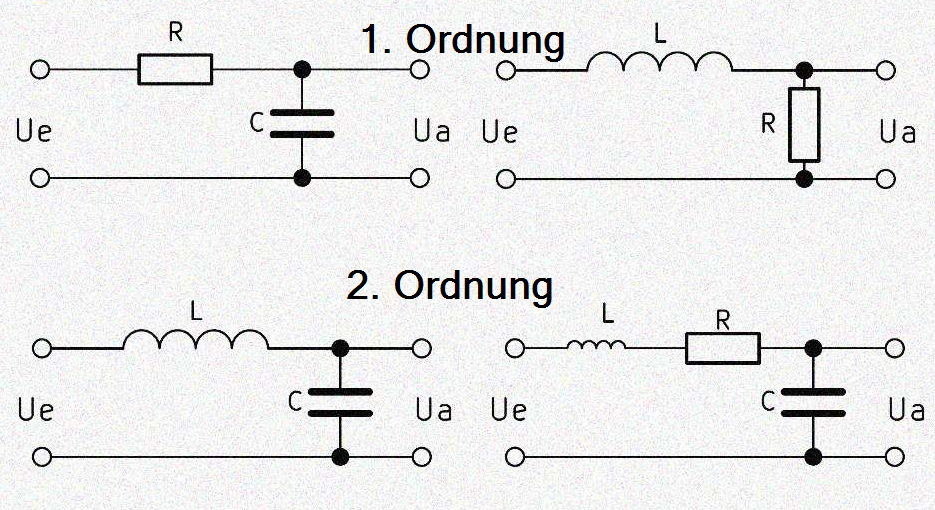
\includegraphics[angle=90,origin=c,width=0.8\linewidth,keepaspectratio=true]{./Images/filter_tiefpass}
\end{minipage}%%% to prevent a space
\begin{minipage}{0.30\textwidth}
	Tiefpass-Filter lässt tiefe Freuenzen durch und filtert hohe raus. Die allgemeine UTF für 1. Ordnung mit RC Komponenten:
	\[
	\frac{1}{\underbrace{RC}_{\tau}s + 1}
	\]
	Der Bode $3dB$ Knick (Real- und Imaginärteil gleich gross, entspricht Phase von $45^\circ$) ist dabei bei $f_{3dB} = \frac{1}{2\pi\tau}$, mit $\tau = RC$
\end{minipage}


\subsection{Sallen Key}
Sallen Key Filter sind nicht geeigenet für hohe Frequenzen, weil Kondensatoren dann wie Kurzschlüsse wirken.
\begin{center}
	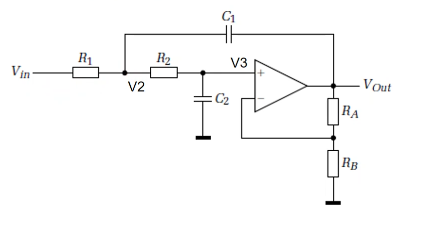
\includegraphics[width=0.7\columnwidth]{Images/sallenkey}
\end{center}
Mit Stromgleichungen kann die UTF dieses Filters bestimmt werden:
\begin{align*}
	0 &= (V_2 - V_{in})\frac{1}{R_1} +(V2 - V3)\frac{1}{R_2} + (V_2 - V_{out})C_1\cdot s \\
	0 &= (V_3 - V_2)\frac{1}{R_2}+ V_3C_2 \cdot s \\
	V_{out} &= \underbrace{\frac{R_A + R_B}{R_B}}_{G_0} \cdot V_3
\end{align*}

\[
H(s) = \frac{G_0}{C_1C_2R_1R_2s^2 + [C_2(R_1 + R_2) + C_1R_1(1 - G_0)]s + 1}
\]
Die Polgüte kann bei kleinen $G_0$ änderungen stark variieren
\begin{align*}
	\omega_0 &= \frac{1}{\sqrt{C_1C_2R_1R_2}} \qquad Q(G_0) &= \frac{\sqrt{C_1C_2R_1R_2}}{C_2(R_1 + R_2) + C_1R_1(1 - G_0) } \\
\end{align*}


\subsection{Multiple Feedback Struktur}
\begin{center}
	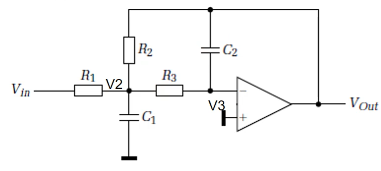
\includegraphics[width=0.7\columnwidth]{Images/multi_feedback}
\end{center}
Der Opamp sorgt für $V_3 = 0$. $C_2$ und $R_1$ kann die Güte angepasst werden. Mit den entsprechenden Stromgleichungen 
\begin{align*}
	0 &= (V_2 - V_{in})\frac{1}{R_1}+(V_2 - V_{out})\frac{1}{R_2} + (V_2 - V_3)\frac{1}{R_3} + V_2C_1s \\
	0 &= (V_3 - V_2)\frac{1}{R_3} + (V_3 - V_{out})C_2s
\end{align*}
ergibt dies eine UTF von
\[
H(s) = \frac{\overbrace{-\frac{R_2}{R_1}}^{G_0}}{C_1C_2R_2R_3s^2 + C_2\left(R_2 + R_3 + R_3\frac{R_2}{R_1}\right)s + 1}
\]
\begin{align*}
	\omega_0 &= \frac{1}{\sqrt{C_1C_2R_2R_3}} \qquad 
	Q(G_0) &= \frac{\sqrt{C_1C_2R_2R_3}}{C_2\left(R_2 + R_3 + R_3\frac{R_2}{R_1}\right) } \\
\end{align*}



\subsection{Zustandsvariablen Filter}
\begin{center}
	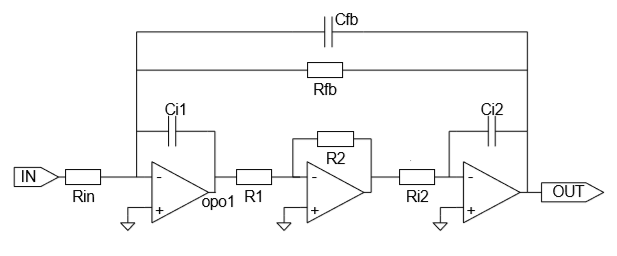
\includegraphics[width=0.7\columnwidth]{Images/zustandsvariablen_filter}
\end{center}
Mit diesem Design können Hoch/Tief und Bandpass Typen erstellt werden
\begin{align*}
	V_{out} &= -\frac{1}{sC_{i2}R_{i2}}V_{opo2} \\
	V_{opo2} &= -\frac{R_2}{R_1}V_{opo1} \\
	V_{opo1} &= \frac{-1}{sC_{i1}}\left(\frac{V_{in}}{R_{in}} + \frac{V_{out}}{R_{fb}} + sC_{fb}V_{out}\right)
\end{align*}

\[
H(s) = \frac{\overbrace{-\frac{R_{rb}}{R_{in}}}^{A_0}}{C_{i1}C_{i2}R_{i2}R_{fb}\frac{R_1}{R_2}\cdot s^2 + C_{fb}R_{fb}\cdot s + 1}
\]
\begin{align*}
	\omega_0 &= \frac{1}{\sqrt{C_{i1}C_{i2}R_{i2}R_{fb}\frac{R_1}{R_2}}} \qquad 
	Q &= \frac{\sqrt{C_{i1}C_{i2}R_{i2}R_{fb}\frac{R_1}{R_2}}}{C_{fb}R_{fb} } \\
\end{align*}


\subsection{Bandpass Filter}
\begin{center}
	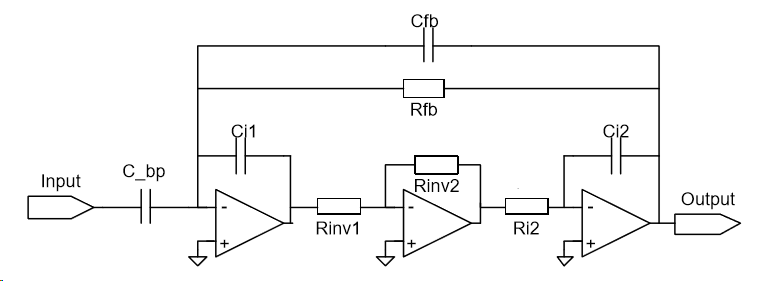
\includegraphics[width=0.6\columnwidth]{Images/bandpass}
\end{center}
Daraus lässt sich die UTF ableiten nach:
\[
H(s) = \frac{-\frac{C_{bp}}{C_{i1}R_{i2}C_{i2}}s}{s^2 + \frac{C_{fb}}{C_{i1}R_{i2}C_{i2}}s + \frac{1}{R_{fb} C_{i1}R_{i2}C_{i2}}}
\]
Die allgemeine Formel für Bandpassfilter lautet
\[
H(s) = \frac{A\cdot\frac{\omega_0}{Q}\cdot s}{s^2 + \frac{ \omega_0}{Q}s + \omega_0^2}
\]

\subsection{Biquad-Filter Struktur}
Können TP, BP und HP-Funktionen erzeugen.
\begin{center}
	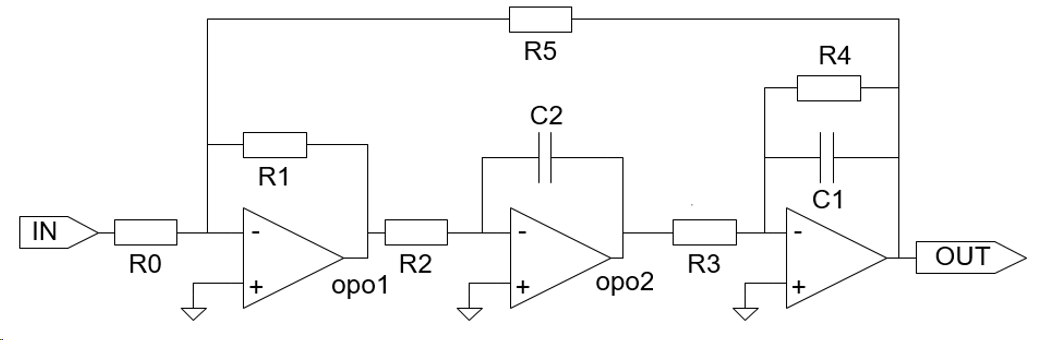
\includegraphics[width=\columnwidth]{Images/biquad}
\end{center}
\[
H(s) = \frac{-\frac{R_5}{R_0}}{C_1C_2R_2R_3\frac{R_5}{R_1}s^2 + \frac{C_2R_2R_3R_5}{R_4R_1}s + 1}
\]

\subsection{Signalflussdiagramm}
\subsubsection{Übertragungsfunktion}
Übertragungsfunktion UTF bestimmt die beziehung zwischem Ein- und Ausgangssignal eines Linearen Dynamischen Systems. UTF von $x_i$ nach $x_j$, wobei $x_i$ eine Quelle, $x_j$ jedoch nicht zwingend eine Senke sein muss wird im allgeminen folgendermassen definiert:
\[
H_{ij} = \frac{\sum_{k} P_{k}\cdot \Delta_k}{\Delta}
\]

\noindent$P_k$: \textbf{Vorwärtspfad} $k$ (start von Eingang): Multiplikation von jeder Sehne von Start bis Ziel\\
$\Delta_k$: \textbf{Kofaktor} des $k$-ten Pfades; 1 - (Summe aller Schleifen die $P_k$ nicht berühren) + (Summe aller Produkte zweier Schleifen, die $P_k$ und sich selbst nicht berühren) - (Summe aller Produkte dreier Schleifen, die $P_k$ und sich selbst nicht berühren) + $\dots$\\
$\Delta$: \textbf{Netzwerkdeterminante}; 1 - (Summe aller Schleifen) + (Summe aller Produkte zweier Schleifen, die sich nicht berühren) - (Summe aller Produktedreier Schleifen, die sich nicht berühren) + $\dots$\\

\noindent\textbf{Beispiel 2. Order Filter}:
\begin{center}
	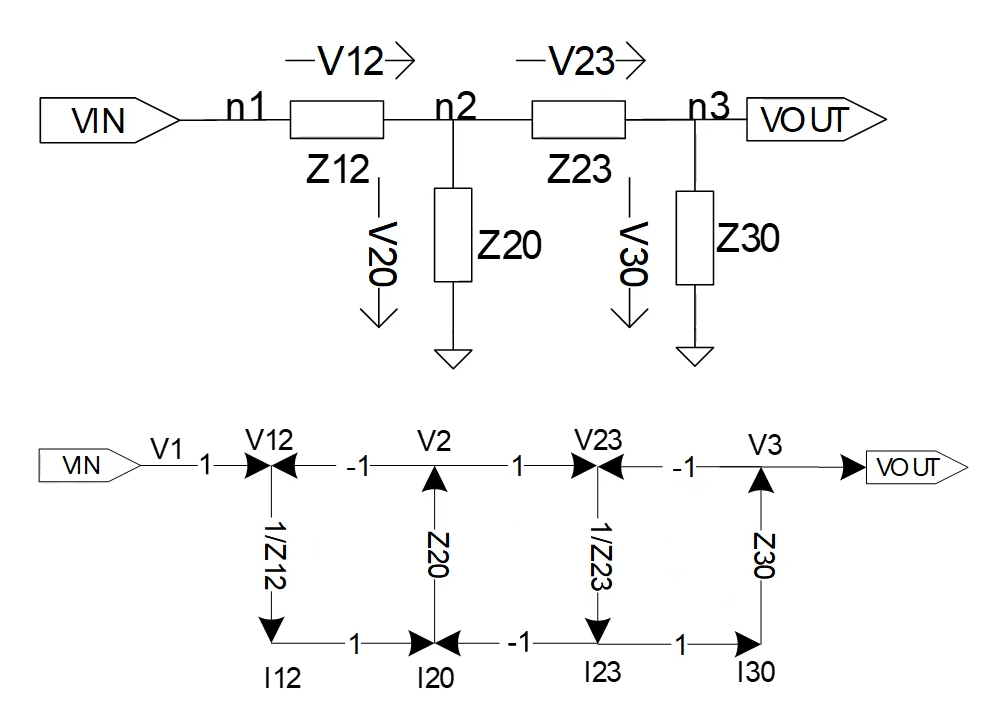
\includegraphics[width=\columnwidth]{Images/sfd}
\end{center}
\[
H(s) = \frac{\frac{Z_{20}}{Z_{12}}\cdot \frac{Z_{30}}{Z_{23}}}{1 + \frac{Z_{20}}{Z_{12}} + \frac{Z_{20}}{Z_{23}} + \frac{Z_{30}}{Z_{23}} + \frac{Z_{20}}{Z_{12}}\cdot\frac{Z_{30}}{Z_{23}} }
\]

\noindent\textbf{Beispiel Bandpass mit SFD}
\begin{center}
	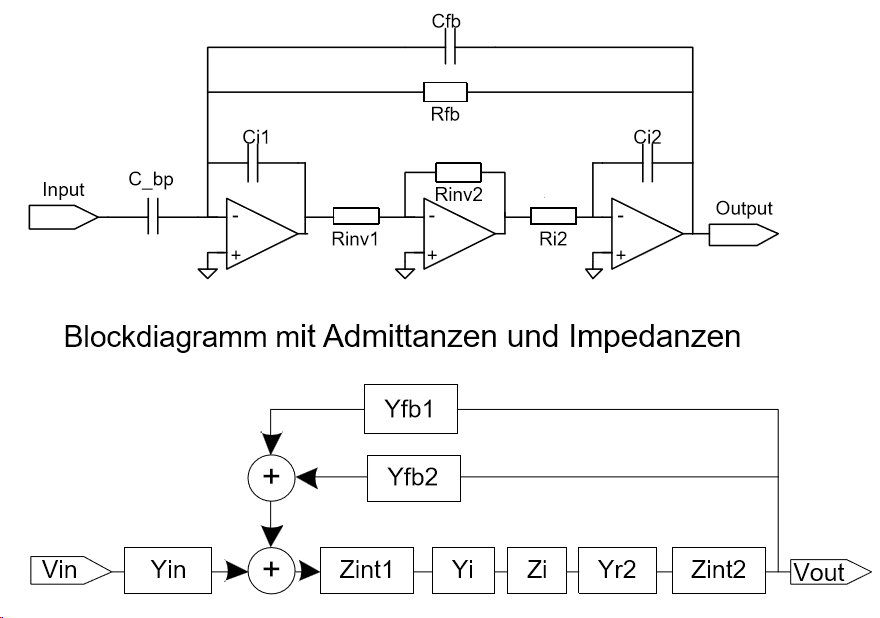
\includegraphics[width=\columnwidth]{Images/bandpass_sfd}
\end{center}
\[
H(s) = \frac{Y_{in}\cdot Z_{int1} \cdot Y_{1} \cdot Z_i \cdot Y_{r1}\cdot Z_{int2}}{1 - (Y_{fb1} + Y_{fb2})\cdot Z_{int1}\cdot Y_{1} \cdot Z_i \cdot Y_{r1}\cdot Z_{int2}}
\]

\subsection{Invertierende Stuktur}
\begin{center}
	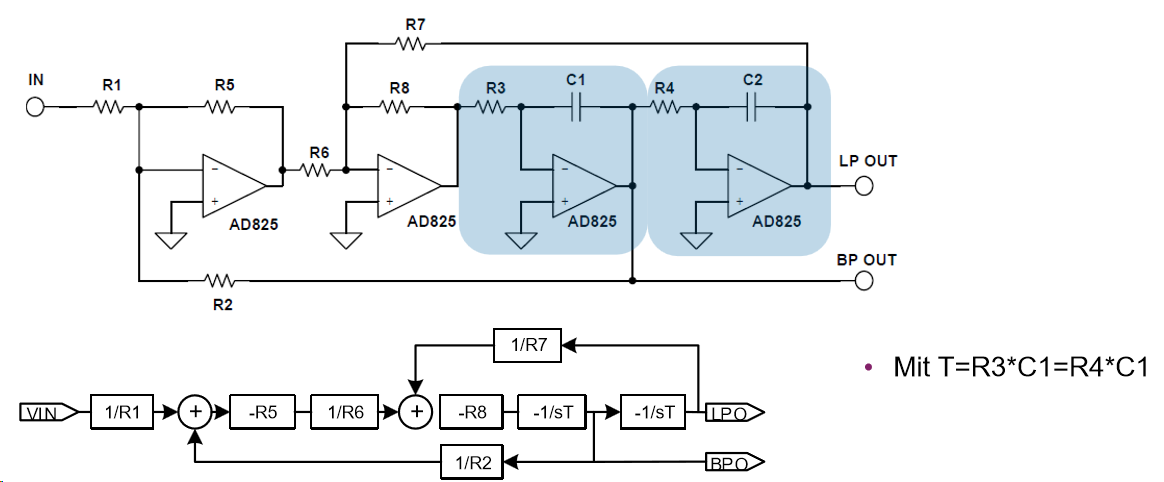
\includegraphics[width=\columnwidth]{Images/invert_filter}
\end{center}
\begin{align*}
	H(s) &= \frac{\frac{-R_5}{R_1}\frac{-R_8}{R_6}\frac{-1}{sT}\frac{-1}{sT}}{1-\frac{-R_5}{R_2}\frac{-R_8}{R_6}\frac{-1}{sT}-\frac{-R_8}{R_7}\frac{-1}{sT}\frac{-1}{sT}} \\
	& = \frac{\frac{R_5R_7}{R_1R_6}}{\frac{R_7}{R_8}T^2s^2 + \frac{R_5R_7}{R_2R_6}Ts + 1}
\end{align*}


\subsection{Oszillator}
Eine UTF schwingt, wenn die Verstärkung $\gt$ 1 und Phase = 0. Damit liegen die Pole auf der Imaginären Achse, D.H wenn Realteil vom UTF Nenner = 0.
\subsubsection{LC}
Nachteil dieser Schaltung ist, dass sie eine bipolare Speisung benötigt.
\begin{center}
	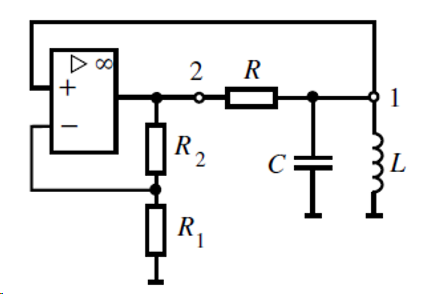
\includegraphics[width=0.4\columnwidth]{Images/lc}
\end{center}
\[
H_{21}(s) = \frac{Ls}{RLCs^2 + Ls +R}
\]

\subsubsection{Pierce-Oszillator}
\begin{center}
	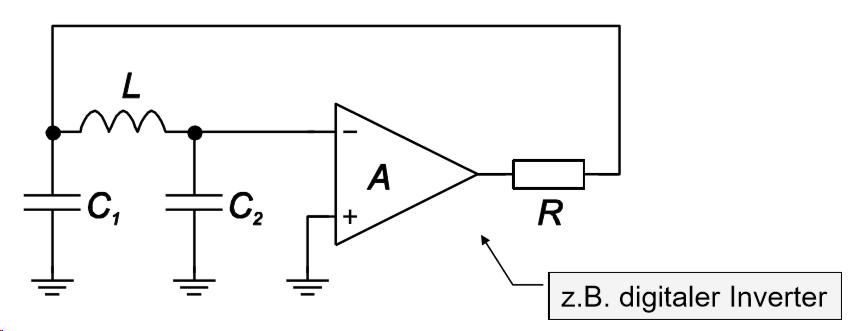
\includegraphics[width=0.6\columnwidth]{Images/piece}
\end{center}
Loop $A(s) \cdot H(s)$:
\[
A \cdot H(s) = \frac{-A}{1 + sR(C_1 + C_2) + s^2LC_2 + s^3RLC_1C_2}
\]
Die Schwingbedingung ist Realteil = 1 (im eingeschwungenen Zustand) und Imaginärteil $0 = j\omega_0R(C_1 + C_2) + (j\omega_0)^3RLC_1C_2$. Die Oszillationsfrequenz ist damit gegeben durch $f_0 = \frac{\omega_0}{2\pi} = \frac{1}{2\pi\sqrt{L\frac{C_1C_2}{C_1 +C_2}}}$. Amplitude $T(\omega_0) = \frac{-A}{1 - \omega_0LC_2} \geq 1$

\subsubsection{Quarz}
\begin{center}
	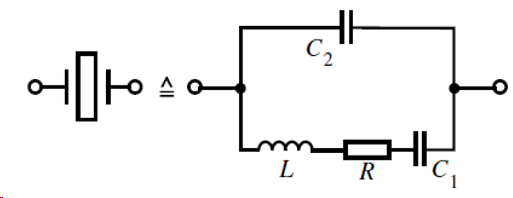
\includegraphics[width=0.6\columnwidth]{Images/quarz}
\end{center}
